\chapter{Introduction}

% Structure:
% - Context
% - Problem
% - Method
% - Results

% - Viele eigene Formate,
% - Nur einen Parser
% - Neue Parser, möglichst schnell implementieren

\section{Motivation \& Problem Statement}

\emph{Parsing} is the process of structuring linear input according to a grammar~\cite{grune2008parsing}. Often the output of this structuring process is a data structure. Research around this topic focuses on how to process the input, how to handle erroneous input and the general computational complexity of algorithms to handle certain kind of \emph{formal languages}.

\begin{figure}[H]
  \centering
    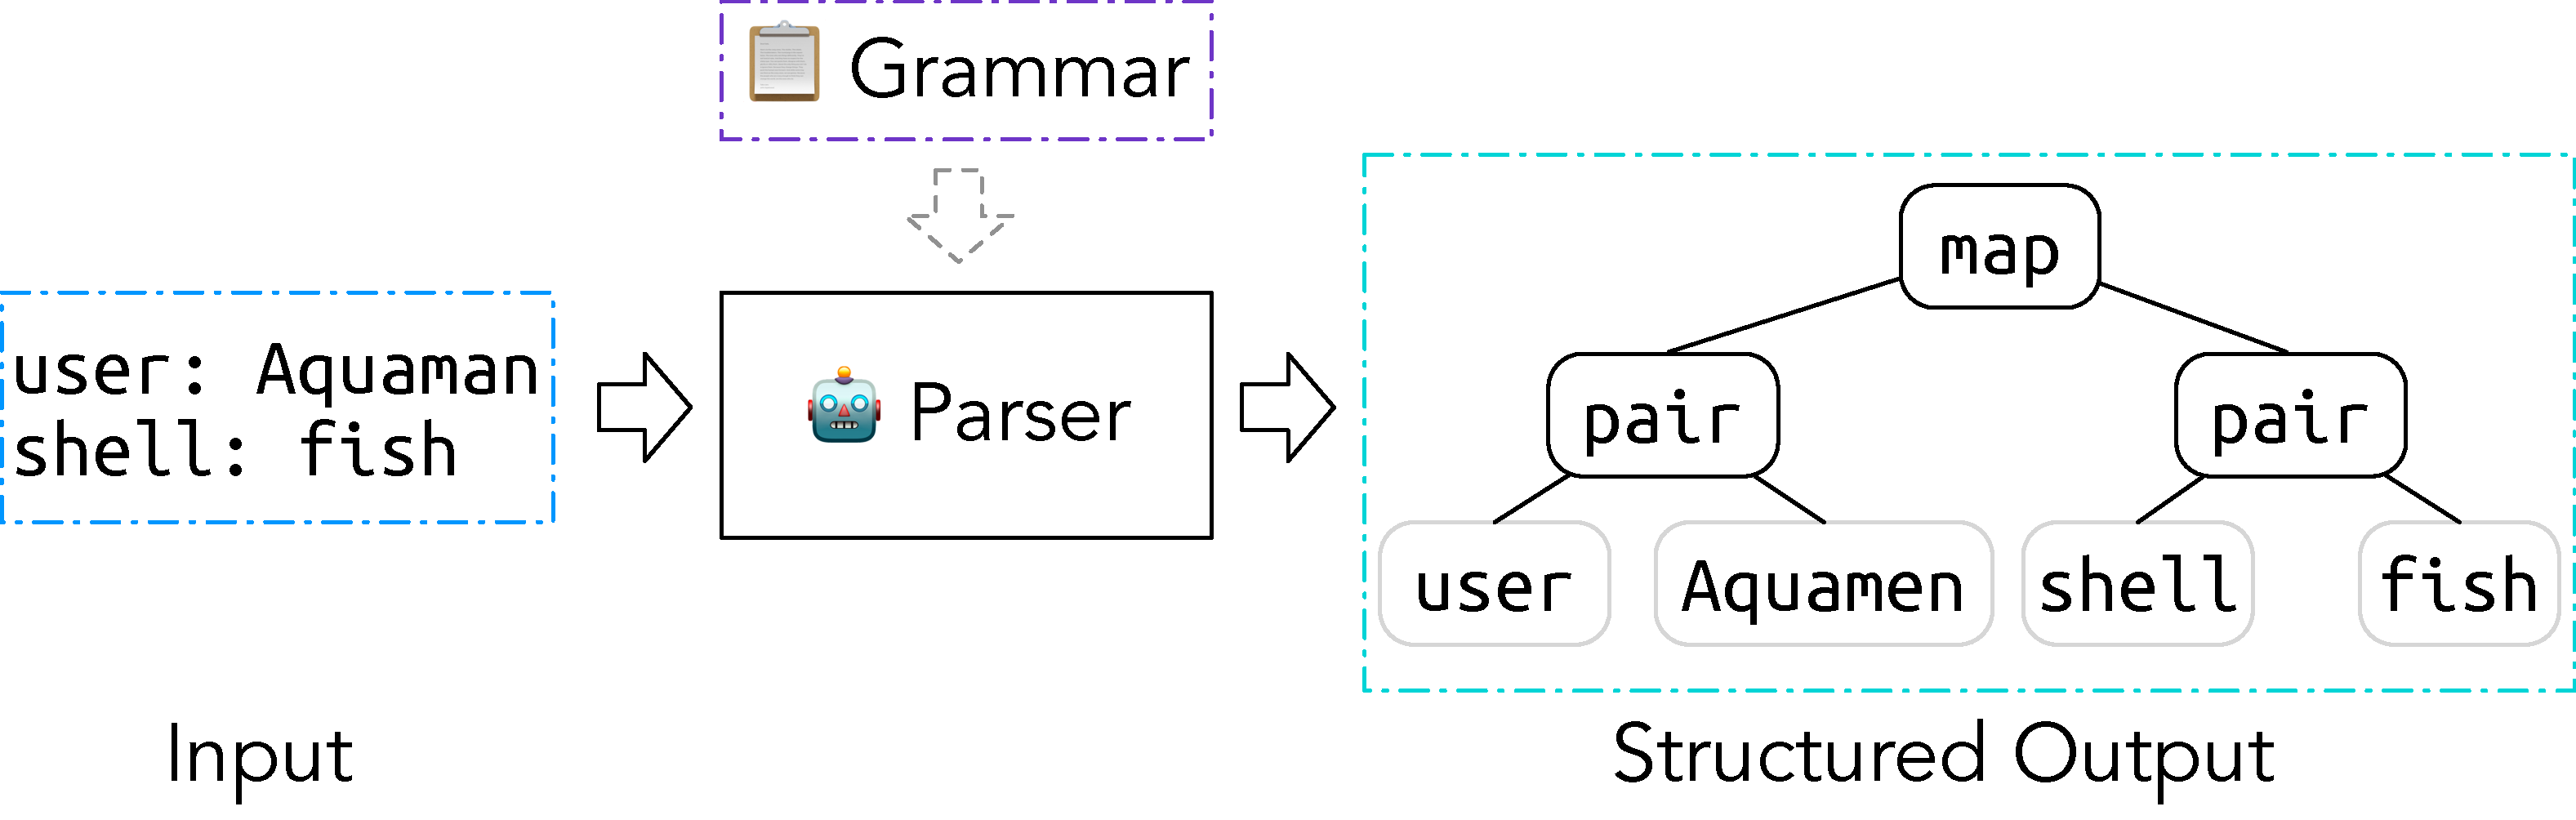
\includegraphics[width=.8\textwidth]{Parsing}
  \caption{Simplified view of the parsing process}
\end{figure}

This thesis concerns itself with the parsing process of languages that are able to express configuration data (e.g. INI, TOML, \glstext{YAML}). These languages form an interesting subpart of formal languages, since accessing key-value based persistent configuration data is a common task for many computer programs.

Just like people disagree about the “best” configuration format, there is currently no consensus, as to which is the ideal way to parse configuration data. There are many possible ways to parse and store data. Notable examples include:

\begin{itemize}
  \item bidirectional programming~\cite{foster2005combinators, bohannon2006relational, lutterkort2008augeas, ko2016bigul, raab2016improving},
  \item code produced by a parser generator~\cite{denny2008ielr, parr2014adaptive, warth2016modular, bates2017aprt},
  \item Serialization libraries~\cite{sumaray2012cds, pacini2015performance}, and
  \item Hand-written parsers~\cite{myers2008cparser, bendersky2012clang}
\end{itemize}

. Currently the possibilities to compare different parsing techniques are limited. The naïve approach would be to just run different parsers on the same data. In practice however, this approach is not usable, since parser tools tend to produce very different data structures. Some of them do not produce data structures at all, instead they let the user specify subroutines that should be called when the parser matches parts of the grammar.

As part of this thesis we will tackle this problem, using different parsing techniques within a common configuration framework. This integration eliminates the problem of comparing the parsing process under different circumstances, since the data structures the parsers create will always be the same. We will use \href{http://web.libelektra.org}{Elektra}, a key-value database, as configuration framework. Elektra’s storage plugin interface will act as foundation for the parsing process. In the end the thesis should provide answers about which parsing techniques provide an ideal balance between performance and usability.

\section{Aim of the Work}
\label{sec:aim_of_the_work}

Ziel besser beschreiben:

Elektra~\cite{raab2010modular, raab2017context} is a plugin based framework that stores configuration parameters in a \gls{KDB}. Elektra reads and stores configuration data via so-called \emph{storage plugins}.

\begin{figure}[H]
  \centering
    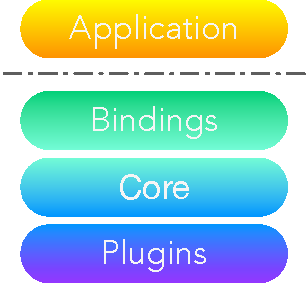
\includegraphics[width=.3\textwidth]{Elektra}
  \caption{Architecture diagram of Elektra}
\end{figure}

As part of this thesis we compare various ways of parsing. For that purpose we wrote and generated parsing code for different storage plugins. All of these storage plugins parse a minimal subset of \glstext{YAML}, a human readable configuration language. We looked at the following parsing technologies:

\begin{itemize}
  \item handwritten parser (recursive descent),
  \item \glstext{ALL(*)} parser generator (\href{http://www.antlr.org}{ANTLR}),
  \item LR parser generator (\href{https://www.gnu.org/software/bison}{Bison}),
  \item Earley parser (\href{https://github.com/vnmakarov/yaep}{YAEP}),
  \item \glstext{PEG} parser (\href{https://github.com/taocpp/PEGTL}{PEGTL}),
  \item parser combinator (\href{https://github.com/orangeduck/mpc}{mpc}), and
  \item bidirectional programming (\href{http://augeas.net}{Augeas})
\end{itemize}

. We compare the parsing code according to the following criteria:

\begin{itemize}
  \item runtime performance,
  \item memory usage,
  \item code size,
  \item overall code complexity,
  \item ease of extensibility and composability, and
  \item error reporting
\end{itemize}

. In the scope of the above comparison we answer the questions below.

\begin{restatable}{question}{speed}
  \label{que:speed}
  How does the theoretic runtime complexity of the parsing methods compare to the actual measured runtime of the parsing code?
\end{restatable}

\begin{restatable}{question}{closeness}
  \label{que:closeness}
  Which parsing technique allows us to stay closest to the definition of the configuration language? Does staying close to the given definition,
  allow us to extend and improve the parser and its support code more easily?
\end{restatable}

\section{Methodological Approach}

The methodological approach for this thesis consists of the steps below.

\begin{description}[style=multiline, leftmargin=3.2cm, font=\bfseries]

  \item[Literature Review] We determined the current status of parsing techniques suitable for configuration file parsing. We then chose appropriate libraries for the parsing techniques listed in the section “\nameref{sec:aim_of_the_work}”.

  \item[Discussion] To determine a minimal usable subset of \glstext{YAML} we discussed common features required for a new Elektra storage plugin with some of the current developers as part of an presentation and subsequent discussion.

  \item[Implementation] We wrote parsing code that handles our minimal \glstext{YAML} subset. In this phase we also added other necessary support code to Elektra.

  \item[Comparison] As noted in “\nameref{sec:aim_of_the_work}” we evaluated the different implementations of our minimal \glstext{YAML} subset parsers.

  \begin{description}
    \item[Runtime Benchmark:] For the runtime comparison we use benchmarks to determine the speed of the different parsing code. In this part of the thesis, we answer \Cref{que:speed}.

    \item[Memory Profiling:] For the memory comparison we use a memory profiling tool to determine the heap memory usage of the \glstext{YAML} plugins.

    \item[Code Count:] We counted the number of code lines with a code line counting tool. This method allow us to consider only actual code, ignoring blank lines and comments.

    \item[Complexity Measurement:] We measured the \gls{CC} of the code using a static analyzer.

    \item[Extensibility \& Composability Check:] To analyze the extensibility and composability of the parsing code we looked at the code difference of commits for certain features and bug fixes. We counted the amount of updated code lines to determine the extension effort. This measurement, together with a comparison between the grammar specification of \glstext{YAML} and the code created in this thesis, will help us to determine the answer for \Cref{que:closeness}.

    \item[Error Reporting:] To determine the quality of the error messages we created erroneous files and compared the quality of the resulting error output.
  \end{description}

\end{description}
